\chapter{The Finite Element Method}

\section{Brief review of the linearized theory of elasticity}
The balance of momentum, stress symmetry and traction definition on the boundary are given by
\begin{equation} \label{eq:pde}
\begin{split}
&{\sigma _{ij,j}} + {f_i} = 0 \quad \forall\ \vec{x} \in V\\
 &\sigma _{ij}=\sigma _{ji}\\
& t_i^{\hat n} = {\sigma _{ij}}{\hat n_{ij}} \quad \forall\ \vec{x} \in S
\end{split} \enspace .
\end{equation}

The simplest constitutive equation in solid mechanics is to consider a linear dependence between stress and strains, and it is called Hooke's law\footnote{Despite the name of \emph{law} used, this relation is not always valid, but is a good approximation for small strains.}
\begin{equation} \label{eq:Hooke}
{\sigma _{ij}} = 2\mu {\varepsilon _{ij}} + \lambda {\varepsilon _{kk}}{\delta _{ij}} \enspace .
\end{equation}

Strain-displacement (kinematic relationship)
\begin{equation}\label{eq:kin}
{\varepsilon _{ij}} = \frac{1}{2}\left( u_{i,j} + u_{j,i}\right)
\end{equation}
\cref{eq:kin} in \cref{eq:Hooke} and the result in \cref{eq:pde} yields
\begin{align*}
\sigma _{ij} &= \mu \left( u_{i,j} + u_{j,i}\right) + \lambda u_{k,k}\delta _{ij}\\
\sigma_{ij,j} &= \mu u_{i,jj} + \mu u_{j,ij} + \lambda u_{k,kj}\delta_{ij}\\
\sigma_{ij,j} &= \mu u_{i,jj} + \left(\lambda  + \mu\right) u_{j,ij}
\end{align*}
from which
\begin{equation} \label{eq:navier}
\begin{split}
&\left(\lambda  + \mu \right)u_{j,ij} + \mu u_{i,jj} + {f_i} = 0 \quad \forall \vec{x} \in V \\
&t_i^{\hat n} = \sigma _{ij} \hat n_{ij} \quad \forall\ \vec{x} \in S_t\\
& {u_i} = \bar{u}_i \quad \forall \vec x \in S_u
\end{split}
\end{equation}

and where ${S_t} \cup {S_u} = S$ and ${S_t} \cap {S_u} = \emptyset $.  

Notice that
\[t_i^{\hat n} =  = \mu \left( {{u_{i,j}} + {u_{j,i}}} \right){{\hat n}_j} + \lambda {u_{k,k}}{\delta _{ij}}{{\hat n}_j} \enspace ,\]
is really a Neumann boundary condition on $u_i$.

\section*{Simple wedge under self-equilibrated loads}
Consider the double wedge of side $\ell$ and internal angle $2 \phi$ shown in \cref{fig:WEDGE}. It is assumed to be contained in the $X-Y$ plane, with loading conditions satisfying a plane strain (or plane stress) idealization. The material is elastic with Lame constants $\lambda$ and $\mu$. The wedge is loaded by uniform tractions of intensity $S$ applied over its four faces in such a way that the wedge is self-equilibrated. We wish to find the closed-form elasticity solution for the stress, strain and displacement fields throughout the problem domain.
%
\begin{figure}[H]
\centering
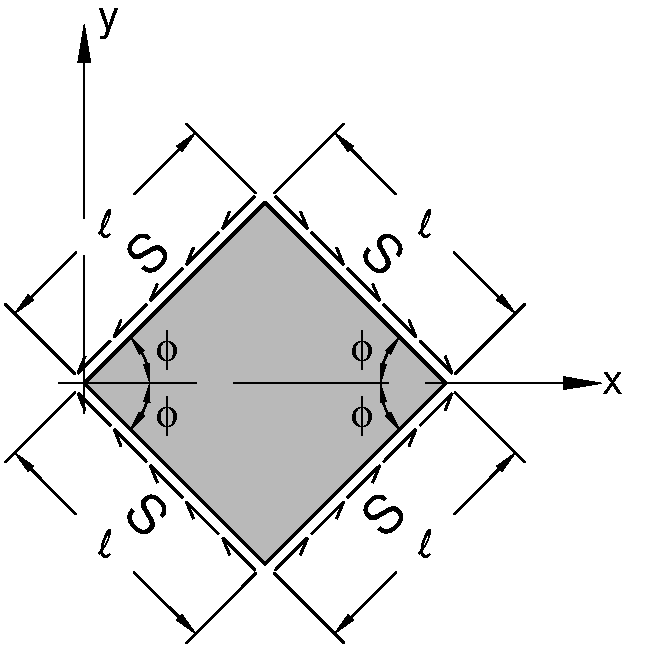
\includegraphics[width=8cm]{img_src/wedge.pdf}
\caption{2D Self-equilibrated wedge.}
\label{fig:WEDGE}
\end{figure}

Under plane strain conditions the general 3D stress equilibrium equations reduce to:
\begin{equation}
\begin{aligned}
&\dfrac{\partial\sigma_{xx}}{\partial x}+\dfrac{\partial\tau_{xy}}{\partial y}=0\\
&\dfrac{\partial\tau_{xy}}{\partial x}+\dfrac{\partial\sigma_{yy}}{\partial y}=0
\end{aligned}
\label{eq:equilibrium}
\end{equation}
with strain given by
\begin{equation}
\begin{aligned}
\epsilon_{xx}&=\dfrac{\partial u}{\partial x}\\
\epsilon_{yy}&=\dfrac{\partial v}{\partial y}\\
\gamma_{xy}&=\dfrac{\partial u}{\partial y} + \dfrac{\partial v}{\partial x}
\end{aligned}
\label{eq:strain}
\end{equation}
where $u$ and $v$ are the horizontal and vertical displacements respectively.

\subsection*{Stress field}

The stress field can be obtained by simple inspection after identifying the traction boundary conditions. In the current problem these conditions correspond to boundary conditions are of the second type given by
\begin{equation}
t_i=\sigma_{ij}\hat{n_j}
\label{eq:bcs}
\end{equation}
and prescribed over the inclined surfaces of the wedge.

Simple equilibrium considerations yield
\begin{align*}
\sum F_x &= 0 \longrightarrow -\ell S\cos(\phi)  + \sigma_{xx}\ell \sin(\phi) = 0\\
\sum F_y &= 0 \longrightarrow -\ell S\sin(\phi) - \sigma_{yy}\ell \cos(\phi)=0
\end{align*}
from which the following stress solution results:
\begin{equation}
\begin{aligned}
\sigma_{xx}& = S \cot(\phi)\\
\sigma_{xx}& = -S\tan(\phi)\\
\tau_{xy}& = 0
\end{aligned}
\label{eq:solution}
\end{equation}
with the condition $\tau_{xy}=0$ due to symmetry.

Let $\hat{n}^1$,  $\hat{n}^2$, $\hat{n}^3$, $\hat{n}^4$ be the outward normal vectors to the exposed faces of the wedge and given by
\begin{align*}
\hat{n}^1 &= -\sin(\phi)\hat{e}_{x}+\cos(\phi)\hat{e}_{y}\\
\hat{n}^2 &= -\sin(\phi)\hat{e}_{x}-\cos(\phi)\hat{e}_{y}\\
\hat{n}^3 &= +\sin(\phi)\hat{e}_{x}+\cos(\phi)\hat{e}_{y}\\
\hat{n}^4 &= +\sin(\phi)\hat{e}_{x}-\cos(\phi)\hat{e}_{y} \enspace .
\end{align*}
The components of the traction vector follow directly like
\[t_{i} = \sigma_{ij}\hat{n}_{j}\]
then over the face with normal $\hat{n}^1$ we have
\begin{align*}
t_{x} &= -S\cos(\phi)\\
t_{y} &= -S\sin(\phi)
\end{align*}
similarly, over the face with normal $\hat{n}^2$
\begin{align*}
t_{x} &= -S\cos(\phi)\\
t_{y} &= +S\sin(\phi)
\end{align*}
over the face with normal $\hat{n}^3$ 
\begin{align*}
t_{x} &= +S\cos(\phi)\\
t_{y} &= -S\sin(\phi)
\end{align*}
and finally, over the face with normal $\hat{n}^4$;
\begin{align*}
t_{x} &= +S\cos(\phi)\\
t_{y} &= +S\sin(\phi) \enspace .
\end{align*}

\subsection*{Strain field}
Using the stress field found in \cref{eq:solution} in the constitutive law for a linear elastic material under plane strain conditions gives us
\begin{equation}
\begin{aligned}
\epsilon_{xx}& = +\dfrac{S}{E}\left[\cot(\phi)+\nu \tan(\phi)\right] = +\dfrac{S}{E}K_{1}(\nu , \phi)\\
\epsilon_{yy}& = -\dfrac{S}{E}\left[\tan(\phi)+\nu \cot(\phi)\right] = -\dfrac{S}{E}K_{2}(\nu , \phi)\\
\gamma_{xy}& = 0.
\end{aligned}
\label{eq:strain part}
\end{equation}

\subsection*{Displacement field}

To determine the displacement field we use the fact that $\omega_{xy}=0$ from which:
\begin{align*}
u &= +\dfrac{S}{E} K_{1}(\nu , \phi)x + A\\
v &= -\dfrac{S}{E} K_{2}(\nu , \phi)y + B
\end{align*}
where $A$ and $B$ are integration constants.

From the condition $u=0$ at $x=l\cos(\phi)$ we have that $A=-\dfrac{S}{E} K_{1}(\nu , \phi)l\cos(\phi)$ then it follows that
\[u=\dfrac{S}{E} K_{1}(\nu , \phi)(x-l\cos(\phi)).\]

Similarly, from the condition $v=0$ at $y=0$ we have that $B=0$ from which
\[v=-\dfrac{S}{E} K_{2}(\nu , \phi)y\]


\section{Formal definition of strong and weak forms}
\subsection*{Strong form}
The strong form of the problem, denoted by $\{ S \}$ reads:\\

Given $f_i$, $t_i^{\hat n}$ and ${\bar u_i}$ find ${u_i}:V \to \Re$ such:
%
\begin{equation} \label{eq:navier_2}
\begin{split}
&\left( {\lambda  + \mu } \right){u_{j,ij}} + \mu {u_{i,jj}} + {f_i} = 0 \quad \text{$\forall \vec x \in V$} \\
&t_i^{\hat n} = {\sigma _{ij}}{\hat n_{ij}} \quad \text{for $\vec x$ in $S_t$}\\
& {u_i} = {{\bar u}_i} \quad \text{for $\vec x$ in $S_u$}
\end{split}
\end{equation}

In \cref{eq:navier_2} the boundary conditions specified by the traction vector $t_i^{\hat n}$ correspond to the natural boundary conditions, while those specified in terms of the displacements vector $\bar u_i$ represent the essential boundary conditions.

\begin{itemize}
\item We are interested in developing methods to obtain approximate solutions to $\{ S \}$.
\item The FEM is formulated starting from a statement equivalent to $\{ S \}$ in which we use trial functions until certain prescribed conditions are met.
\item We will look for solutions $u_i$ subject to the following conditions:

\begin{align*}
u_i=\bar u_i\\
\int\limits_S {{{\left( {\frac{{\partial {u_i}}}{{\partial {x_j}}}} \right)}^2}} dS < \infty
\end{align*}

\end{itemize}

The first condition corresponds to the satisfaction of the essential boundary condition, while the second corresponds to the functions being square integrable. The space of functions satisfying the above two conditions is denoted by $\varsigma$ and formally defined like;

\[ \varsigma = \left\{ {{u_i}\left| {{u_i} \in H,{u_i} = {{\bar u}_i} \quad in \quad {S_u}} \right.} \right\}\].

On the other hand, in order to validate the introduced trial functions we also need testing (or weighting and distribution) functions $w_i$. Such functions are arbitrary apart form having to satisfy the following conditions:

\[w_i=0 \quad in \quad {S_u}\]

\[\int\limits_S {{{\left( {\frac{{\partial {w_i}}}{{\partial {x_j}}}} \right)}^2}} dS < \infty \]

In what follows we formally denote the space of these functions by $V$ and formally define it like

\[ V = \left\{ {{w_i}\left| {{w_i} \in H,{u_i} = {w_i=0} \quad in \quad {S_u}} \right.} \right\}\]

\subsection*{Weak form}
Having defined the strong form $\{S\}$ and the spaces $\varsigma$ and $V$ we will state an alternative form (equivalent to $\{S\}$) but with advantages when thinking about a numerical solution. Since in that form the continuity requirements of the trial functions is weaker than in the strong form such formulation is commonly referred to like the weak form $\{W\}$ and defined as follows.

Given $f_i$, $t_i^{\hat n}$ and ${\bar u_i}$ find ${u_i}:V \to \Re$ and $\forall {w_i} \in V$ such:

\[\int\limits_V {{\sigma _{ij,j}}{w_{i,j}}dV - \int\limits_V {{f_i}{w_i}dV}  - \int\limits_{{S_t}} {t_i^{\hat n}} } {w_i}dS = 0\]

\subsubsection*{Proof 1:}
Let $u_i \in \varsigma $ be a solution to $\{S\}$ and let $w_i \in V $. Forming the inner product of the equilibrium statement with $w_i$ and forcing the integral over the domain to be zero we have:

\[\int\limits_V {\left( {{\sigma _{ij,j}} + {f_i}} \right){w_i}} dV = 0\]

expanding the terms in the integrand yields;

\[\int\limits_V {{\sigma _{ij,j}}{w_i}dV + \int\limits_V {{f_i}{w_i}dV = 0} } \]

Now integrating by parts the first term on the left we have:

\[ - \int\limits_V {{w_{i,j}}{\sigma _{ij}}dV}  + \int\limits_S {{\sigma _{ij}}{{\hat n}_j}{w_i}dS}  + \int\limits_V {{w_i}{f_i}dV = 0} \]

since $w_i \in V$ it follows that $w_i = 0$ in $S_u$ from which

\begin{equation}\label{weak}
\int\limits_V {{\sigma _{ij,j}}{w_{i,j}}dV - \int\limits_V {{f_i}{w_i}dV}  - \int\limits_{{S_t}} {t_i^{\hat n}} } {w_i}dS = 0
\end{equation}


Now, considering that $u_i$ is solution of the strong form $\{S\}$ it must satisfy $u_i = \bar u_{i} \quad in \quad S_u$ and as a result $u_i \in \varsigma$. On the other hand, since $u_i$ satisfies \cref{weak} $\forall {w_i} \in V$ we have that $u_i$ satisfies the definition of weak solution specified in $\{ W \}$.

\subsubsection*{Proof 2:}
Let $u_i$ be a solution of $\{W\}$ and thus $u_i \in \varsigma$ which means that:

\[u_i = \bar u_{i} \quad in \quad S_u\]

and that it satisfies

\[\int\limits_V {{\sigma _{ij}}{w_{i,j}}dV - \int\limits_V {{f_i}{w_i}dV - \int\limits_{{S_t}} {t_i^n} } } {w_i}dS = 0\]

integrating by parts,

\[ - \int\limits_V {{\sigma _{ij,j}}{w_i}dV + \int\limits_S {{\sigma _{ij}}{n_j}{w_i}}  - \int\limits_V {{f_i}{w_i}dV - \int\limits_{{S_t}} {t_i^n} } } {w_i}dS = 0\]

Since ${w_i} \in V$ we have that ${w_i}=0$ in $S_u$ and therefore:

\[\int\limits_V {{w_i}\left( {{\sigma _{ij,j}} + {f_i}} \right)dV + \int\limits_{{S_t}} {{w_i}\left( {{\sigma _{ij}}{n_j} - t_i^n} \right)dS = 0} } \]

from which:

\begin{equation} \label{equil_2}
\begin{split}
&{\sigma _{ij,j}} + {f_i} = 0 \quad \vec{x} \in V \\
&t_i^n = {\sigma _{ij}}{n_j} \quad for \quad \vec{x} \quad in \quad S_t\\
&{u_i} = {{\bar u}_i} \quad for \quad \vec{x} \quad in \quad S_u
\end{split}
\end{equation}

\subsection{The principle of virtual work-Discretization into local interpolating functions}
We now discretize the principle of virtual work repeated below for completeness:

\begin{equation} \label{pvw_2}
\int\limits_V {{\sigma _{ij}}\delta {u_{i,j}}dV - \int\limits_V {{f_i}\delta {u_i}dV - \int\limits_{{S_t}} {t_i^n} } } \delta {u_i}dS = 0.
\end{equation}

For that purpose we will divide the complete domain $V$ into $N$-finite non-overlapping subdomains over each one of which we will approximate the solution in terms of local interpolating functions. Since the PVW (or weak form of the BVP) has been casted into an integral representation, it is possible to build the total integral considering the contribution of the $N$-sub-domains as follows;

\begin{equation}\label{pvw_dis}
\sum\limits_{e = 1}^{NEL} {\int\limits_{{V^e}} {{\sigma _{ij}}\delta {u_{i,j}}d{V^e} - \int\limits_V {{f_i}\delta {u_i}d{V^e} - \int\limits_{{S_t}} {t_i^n} } } \delta {u_i}d{S^e} = 0} 
\end{equation}

For easiness consider a single subdomain

\begin{equation} \label{pvw_sing}
\int\limits_V {{\sigma _{ij}}\delta {u_{i,j}}dV - \int\limits_V {{f_i}\delta {u_i}dV - \int\limits_{{S_t}} {t_i^n} } } \delta {u_i}dS = 0.
\end{equation}

The involved functions (e.g., displacements, strain, stresses) will be approximated via interpolation of the solution over a determined number of points termed in what follows nodes. Assume for instance that over element $e$ containing $n$ such nodes we know the displacements vector $u_i$. Furthermore, let the displacements for the $p$-node $u^P=[u^P, v^P, w^P]$. Using ideas from interpolation theory it is now possible to approximate the displacements vector over an arbitrary point $\vec{x}$ inside the element as follows;

\[{u_i}(\vec x) = N_i^1(\vec x){u^1} + N_i^2(\vec x){u^2} + ... + N_i^P(\vec x){u^P} + ... + N_i^n(\vec x){u^n}\]

or in more general form;

\begin{equation} \label{bas_interpol}
{u_i}(\vec x) = N_i^Q(\vec x){u^Q}
\end{equation}

and where the caption superscripts indicate summation over the number of nodes of the element while the subscript refers to the physical character of the variable being interpolated.

\[{\varepsilon _{ij}}(\vec x) = B_{ij}^Q(\vec x){u^Q}\]

\[{\varepsilon _{ij}}(\vec x) = \frac{1}{2}\left( {{u_{i,j}} + {u_{j,i}}} \right)\]


\[{\varepsilon _{ij}}(\vec x) = \frac{1}{2}\left( {\frac{{\partial N_i^Q}}{{\partial {x_j}}} + \frac{{\partial N_j^Q}}{{\partial {x_i}}}} \right){u^Q}\]

\[B_{ij}^Q = \frac{1}{2}\left( {\frac{{\partial N_i^Q}}{{\partial {x_j}}} + \frac{{\partial N_j^Q}}{{\partial {x_i}}}} \right)\]

\[\delta {u_i} = N_i^Q(\vec x)\delta {u^Q}\]

\[\int\limits_V {{C_{ijkl}}B_{kl}^P{u^P}B_{ij}^Q\delta {u^Q}dV - \int\limits_V {{f_i}N_i^Q\delta {u^Q}dV}  - \int\limits_{{S_t}} {t_i^nN_i^Q\delta {u^Q}dS = 0} } \]

\[\delta {u^Q}\int\limits_V {B_{ij}^Q{C_{ijkl}}B_{kl}^PdV{u^P} - \delta {u^Q}\int\limits_V {N_i^Q{f_i}dV}  - \delta {u^Q}\int\limits_{{S_t}} {N_i^Qt_i^ndS = 0} } \]

\[\delta {u^Q}f_\sigma ^Q - \delta {u^Q}f_V^Q - \delta {u^Q}f_c^Q = 0\]

\[f_\sigma ^Q - f_V^Q - f_c^Q = 0\]

\[f_\sigma ^Q = \int\limits_V {B_{ij}^Q{C_{ijkl}}B_{kl}^PdV{u^P} \equiv {K^{QP}}} {u^P}\]

\[f_V^Q = \int\limits_V {N_i^Q{f_i}dV} \]

\[f_c^Q = \int\limits_{{S_t}} {N_i^Qt_i^ndS} \]

\[{K^{QP}}{u^P} = f_V^Q + f_c^Q\]

\section[Discretization of the PVW using FEM]{Discretization of the PVW via the FEM}

\subsection*{Application to a simple spring-mass system}


\begin{algorithm}[H]
 \SetAlgoLined
 \KwData{Problem paramters; NUMNP, NUMEL, NMATP}
 \KwResult{Displacements and spring forces}
 Create $DM$E operator\;
 Assemble $K^G$, $F^G$\;
\While{$j \leq 1, NUMEL$}{
\[
\begin{aligned}
K^G \leftarrow K^G+K^i\\
F^G \leftarrow F^G+F^i\\
\end{aligned}
\]
}
Impose BCs\;
Solve $[K^G]U=F^G$\\
Find internal forces
\caption{Springs Algorithm}
\end{algorithm}


\section{Variational formulations}
\todo{Add Variational formulation definition.}
According to Wikipedia \cite{wiki:variational_principle}

\begin{quotation}
A variational principle is a scientific principle used within the calculus of variations, which develops general methods for finding functions which minimize or maximize the value of quantities that depend upon those functions. For example, to answer this question: ``What is the shape of a chain suspended at both ends?" we can use the variational principle that the shape must minimize the gravitational potential energy.

According to Cornelius Lanczos, any physical law which can be expressed as a variational principle describes an expression which is self-adjoint. These expressions are also called Hermitian. Such an expression describes an invariant under a Hermitian transformation.
\end{quotation}

\subsection{Principle of minimum potential energy}

\subsection{Hu-Washizu Variational Principle}
Consider the following functional
\begin{equation}
{\pi ^*} = \pi  - \int\limits_V {\lambda _{ij}^\varepsilon ({\varepsilon _{ij}} - {L_{ijk}}{u_k})dV}  - \int\limits_{{S_u}} {\lambda _i^u(u_i^{{S_u}} - {{\bar u}_i})dS}
\label{eq:Hu}
\end{equation}
where
\begin{itemize}
\item $\pi$: is the potential energy functional.
\item $L_{ijk}$ is a differential operator such ${\varepsilon _{ij}} = {L_{ijk}}{u_k}$.
\item $S_u$ surface where essential boundary conditions are prescribed.
\item $\lambda _{ij}^\varepsilon $ and ${\lambda _i^u}$ are Lagrange multipliers.
\end{itemize}

We want to determine the so-called Euler equations resulting from the condition $\delta \pi^* = 0$. Applying the variational operator we have:
\begin{equation}
\begin{aligned}
\delta \pi *& = \delta \pi  - \int\limits_V {\delta \lambda _{ij}^\varepsilon } ({\varepsilon _{ij}} - {L_{ijk}}{u_k})dV- \int\limits_V {\lambda _{ij}^\varepsilon } (\delta {\varepsilon _{ij}} - {L_{ijk}}\delta {u_k})dV \\
&-\int\limits_V {\delta \lambda _i^u} (u_i^{{S_u}} - {\bar u_i})dS - \int\limits_V {\lambda _i^u} \delta u_i^{{S_u}}dS
\end{aligned}
\end{equation}

\begin{equation}
\begin{aligned}
\delta \pi * &= \int\limits_V {{C_{ijkl}}{\varepsilon _{kl}}\delta {\varepsilon _{ij}}dV - \int\limits_{{S_t}} {{t_i}\delta {u_i}dS}  - \int\limits_V {{f_i}\delta {u_i}dV - } }\int\limits_V {\lambda _{ij}^\varepsilon \delta {\varepsilon _{ij}}dV}  + \int\limits_V {\lambda _{ij}^\varepsilon {L_{ijk}}\delta {u_k}dV}\\
&- \int\limits_V {\delta \lambda _{ij}^\varepsilon ({\varepsilon _{ij}} - {L_{ijk}}{u_k})dV - \int\limits_S {\delta \lambda _i^u(u_i^{{S_u}} - {{\bar u}_i})dS - \int\limits_{{S_u}} {\lambda _i^u\delta {u_i}dS = 0} } }
\end{aligned}
\end{equation}

using

\[\int\limits_V {(\lambda _{ij}^\varepsilon \delta {u_i}){,_j}dV = } \int\limits_V {\lambda _{ij}^\varepsilon \delta {u_{i,j}}dV}  + \int\limits_V {\lambda _{ij,j}^\varepsilon \delta {u_i}dV} \]

in the above we can write

\begin{align*}
\int\limits_V {\lambda _{ij}^\varepsilon {L_{ijk}}\delta {u_k}dV} & = \int\limits_V {{{(\lambda _{ij}^\varepsilon \delta {u_i})}_{,j}}dV}  - \int\limits_V {\lambda _{ij,j}^\varepsilon \delta {u_i}dV}\\
& = \int\limits_{{S_t}} {\lambda _{ij}^\varepsilon \delta {u_i}{{\hat n}_j}dS}  - \int\limits_V {\lambda _{ij,j}^\varepsilon \delta {u_i}dV}
\end{align*}

therefore


\begin{align*}
\delta \pi * &= \int\limits_V {({C_{ijkl}}{\varepsilon _{kl}} - \lambda _{ij}^\varepsilon )\delta {\varepsilon _{ij}}dV - \int\limits_{{S_t}} {{t_i}\delta {u_i}dS}  - \int\limits_V {{f_i}\delta {u_i}dV + } } \int\limits_{{S_t}} {\lambda _{ij}^\varepsilon \delta {u_i}{{\hat n}_j}dS}  - \int\limits_V {\lambda _{ij,j}^\varepsilon \delta {u_i}dV}\\
&- \int\limits_V {\delta \lambda _{ij}^\varepsilon ({\varepsilon _{ij}} - {L_{ijk}}{u_k})dV}  - \int\limits_{{S_u}} {\delta \lambda _i^u(u_i^{{S_u}} - {{\bar u}_i})dS}  - \int\limits_{{S_u}} {\lambda _i^u\delta {u_i}dS}  = 0
\end{align*}


\begin{align*}
&\int\limits_V {({C_{ijkl}}{\varepsilon _{kl}} - \lambda _{ij}^\varepsilon )\delta {\varepsilon _{ij}}dV
+ \int\limits_{{S_t}} {(\lambda _{ij}^\varepsilon {{\hat n}_j} - {t_i})\delta {u_i}dS}  - }\\
&\int\limits_V {(\lambda _{ij,j}^\varepsilon  + {f_i})\delta {u_i}dV}
- \int\limits_V {({\varepsilon _{ij}} - {L_{ijk}}{u_k})\delta \lambda _{ij}^\varepsilon dV}
- \int\limits_{{S_u}} {(u_i^{{S_u}} - {{\bar u}_i})\delta \lambda _i^udS}  - \cancel{\int\limits_{{S_u}} {\lambda _i^u\delta u_i^{{S_u}}dS} = } 0
\end{align*}


Now, imposing the conditions $\delta {\varepsilon _{ij}} \neq 0$, $\delta \lambda _{ij}^\varepsilon  \neq 0$, $\delta {u_i} \neq 0$ in $S_t$, $\delta {u_i} \neq 0$ in $V$ and $\delta \lambda _i^u \neq 0$ in $S_u$ we have
%
\begin{align}
&\lambda _{ij}^\varepsilon  = C_{ijkl} \varepsilon_{kl}\\
&\varepsilon_{ij} = {L_{ijk}}{u_k}\\
t_i &= \lambda_{ij}^\varepsilon \hat{n}_j\\
&\lambda _{ij,j}^\varepsilon  + {f_i} = 0\\
&u_i^{S_u} = \bar{u}_i
\end{align}

\section{Weighted residual methods}
\subsection{Application to the Navier equations}
\subsection{Application to the acoustic wave equation}

\section{Basic elements of interpolation theory}
\subsection{Formulation in the physical space}
\subsection{Formulation in the natural space: the continuum mechanics analogy}
In typical finite element equilibrium equations we need to perform integration over the reference element domain $V_0(\vec{x})$ corresponding to originally arbitrarily shaped sub-domains as created during the meshing process.  In order to proceed with this integration it is useful to consider the following continuum mechanics analogy.

First assume that the actual physical domain $V_0(\vec{x})$ is the result of a deformation process imparted upon the natural domain as shown in \cref{fig:natural domain}. In this analogy, the physical domain $V_0(\vec{x})$ is regarded like a ``deformed'' configuration at an imaginary time $t=t$, while the natural ``undeformed'' domain $V(\vec{r})$   is treated like a reference undeformed configurations at time $t=0$. Both configurations are assumed to be connected through a deformation process;


\begin{equation}
\begin{aligned}
\vec{X}&=\vec{X}(\vec{r})\\
\vec{r}&=\vec{r}(\vec{X})
\end{aligned}
\label{eq:motion}
\end{equation}

\begin{figure}[h]
\centering
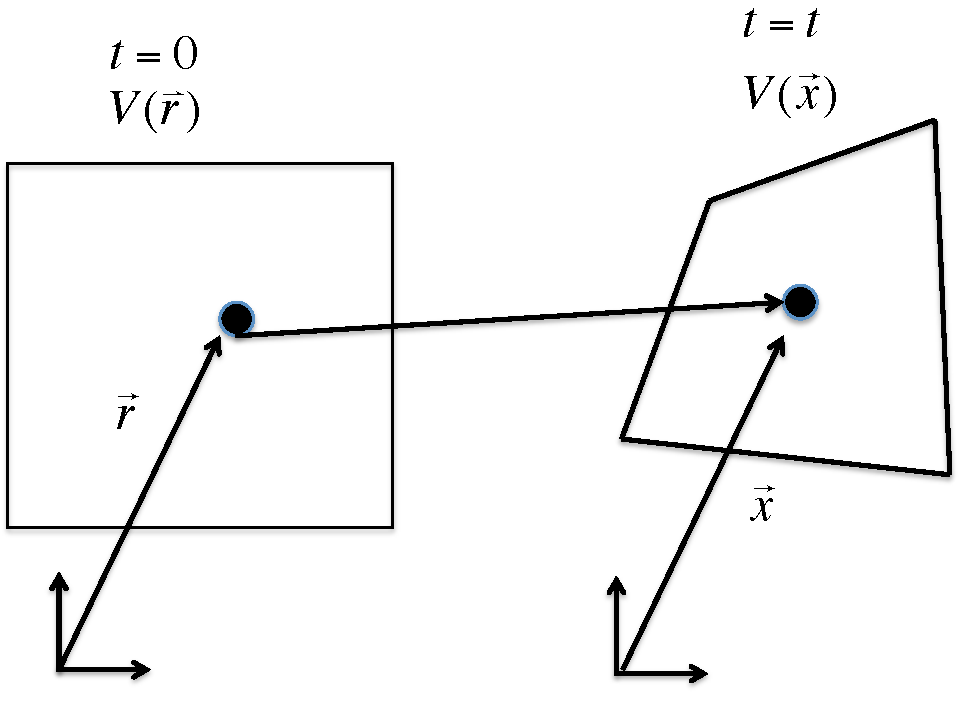
\includegraphics[width=8cm]{img/figure1.pdf}
\caption{Definition of the natural domain}
\label{fig:natural domain}
\end{figure}

 

In \cref{eq:motion} we can understand $\vec{r}$ like a material (Lagrangian) variable and $\vec{X}$ like a spatial (or Eulerian) variable. Using the continuum mechanics analogy it is clear that the ``deformation'' process at the continuum level is fully characterized by the ``deformation'' gradient or Jacobian of the transformation \cref{eq:motion} and defined according to;

\begin{equation}
dX_i=\dfrac{\partial X_i}{\partial r_J}dr_J\equiv J_{iJ}dr_{J}
\label{eq:gradient}
\end{equation}

where $dr_{J}$ and $dX_i$ represent material vectors in the original and deformed configuration. From \cref{eq:gradient} it is evident that the Jacobian contains all the information describing the change of the physical sub-domain with respect to the natural element. For the element integration process we will assume that every element $V(\vec{r})$ in the natural domain deforms into the physical element $V_0(\vec{X})$, thus allowing us to write typical terms like the ones in the material stiffness matrix
\begin{equation}
\int\limits_{V(\vec{X})} \hat{B}_{ij}^K(\vec{X}) C_{ijkl} \hat{B}_{kl}^P(\vec{X}) dV(\vec{X})\equiv \int\limits_{V_0(\vec{r})} \hat{B}_{ij}^K(\vec{r}) C_{ijkl} \hat{B}_{kl}^P(\vec{r})J dV_0(\vec{r})
\label{eq:matmatrix}
\end{equation}
where we have used $dV(\vec{X})=JdV(\vec{r})$, with $J$ being the determinant of the deformation gradient and in general we transform functions between the natural and physical space making use of \cref{eq:motion} according to
\begin{equation}
f(\vec{r})=F[\vec{X}(\vec{r})]
\label{eq:funtrans}
\end{equation}

	 								
\section*{Interpolation scheme}
Having identified the fact that the integration process will take place in the natural domain, we will approach the interpolation process directly in this natural space. In the case of the displacement based finite element method all the involved variables will then be obtained via interpolation of nodal displacements. For instance, assume that a given problem variable is defined in the physical space by the tensor $\Phi_{ik...p}(\vec{X})$. The interpolated variable is then written like;

\begin{equation}
\Phi_{ij...p}(\vec{X})=H_{ij...p}^K(\vec{r})\hat{u}^K
\label{eq:interpol}
\end{equation}	 						

where $\hat{u}^K$ represents a vector of nodal points displacements, see \cref{fig:interpol nat dom}, and $H_{ij...p}^K(\vec{r})$ is an interpolator which keeps the tensorial character of the original physical variable $\Phi_{ik...p}(\vec{X})$ and where the super-index makes reference to a nodal identifier (with the summation convention in place).


\begin{figure}[h]
\centering
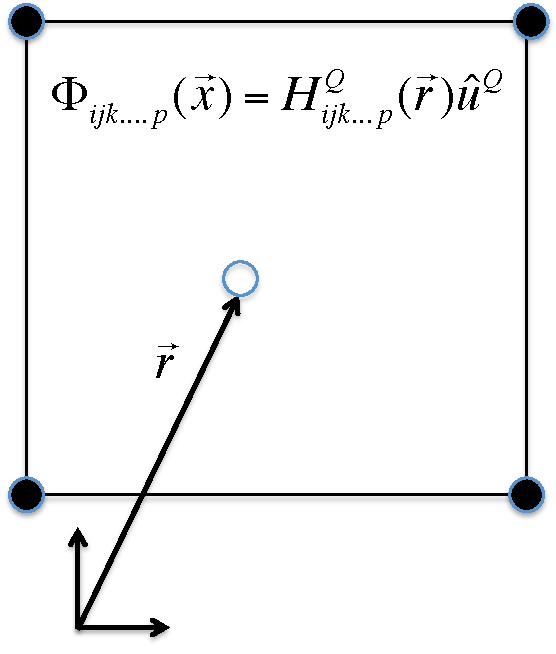
\includegraphics[width=4cm]{img/figure2.pdf}
\caption{General interpolation strategy in the natural domain}
\label{fig:interpol nat dom}
\end{figure}
 


Since the primary variable corresponds to displacements it must be kept in mind that $H_{ij...p}^K(\vec{r})$ corresponds to combinations of derivatives (or other arbitrary combinations) of the basic element shape functions defined in;


\begin{equation}
u_i(\vec{X})=N_i^K(\vec{r})\hat{u}^K
\label{eq:el interpol}
\end{equation}



For the general interpolation process we need two kinds of transformations.  First we need to transform integrals over the physical space into integrals into the natural space which corresponds to
\begin{equation}
\int\limits_{V(\vec{X})} F(\vec{X})dV(\vec{X})\equiv \int\limits_{V_0(\vec{r})} f(\vec{r})J dV_0(\vec{r})
\label{gen trans}
\end{equation}



Second we need to relate spatial differentiation in both, the physical and spatial domains.  Let us define these operators like $\nabla_i^X$ and $\nabla_I^r$ respectively. It then follows from \cref{eq:funtrans} that
\begin{equation}
\dfrac{\partial F}{\partial X_i}=\dfrac{\partial f}{\partial r_J}\dfrac{\partial r_J}{\partial X_i}
\label{eq:chain}
\end{equation}
from where we can establish the connection between the two operators like


\begin{equation}
\nabla_i^X=J_{iJ}^{-1}\nabla_J^r
\label{eq:fundamental}
\end{equation}


\section*{The fundamental interpolator}
We further define the fundamental interpolator giving rise to gradients of the primary displacement variable in the physical space according to
\begin{equation}
u_{i,j}(\vec{X})=L_{ij}^K(\vec{r})\hat{u}^K
\label{eq:fund operator}
\end{equation}


This fundamental interpolator  $L_{ik}^K(\vec{r})$ is derived after using \cref{eq:el interpol} and \cref{eq:fundamental} in the physical displacement gradient definition as shown next
\begin{align*}
u_{i,j}(\vec{X})&=\nabla_j^X u_i(\vec{X})\\
u_{i,j}(\vec{X})&=\nabla_j^X N_i^K(\vec{r})\hat{u}^K\\
u_{i,j}(\vec{X})&=J_{jQ}^{-1}\nabla_Q^r N_i^K(\vec{r})\hat{u}^K\\
u_{i,j}(\vec{X})&=J_{jQ}^{-1}N_{i,Q}^K(\vec{r})\hat{u}^K
\end{align*}
then
\begin{equation}
L_{ij}^K(\vec{r})=J_{jQ}^{-1}N_{i,Q}^K(\vec{r})
\label{eq:fundamental interpolator}
\end{equation}

\section*{Elemental stiffness matrix}
The elemental material stiffness matrix computed in the natural domain of \cref{fig:Nat domain} reads;

\begin{equation}
K^{KP}=\int\limits_{V_0(\vec{r})} \hat{B}_{ij}^K(\vec{r}) C_{ijkl} \hat{B}_{kl}^P(\vec{r})J dV_0(\vec{r})\equiv \int\limits_{r=-1}^{r=+1}\int\limits_{s=-1}^{s=+1} \hat{B}_{ij}^K(r,s) C_{ijkl} \hat{B}_{kl}^P(r,s)J(r,s) \mathrm{d}r\mathrm{d}s
\label{eq:elematrix}
\end{equation}



\begin{figure}[h]
\centering
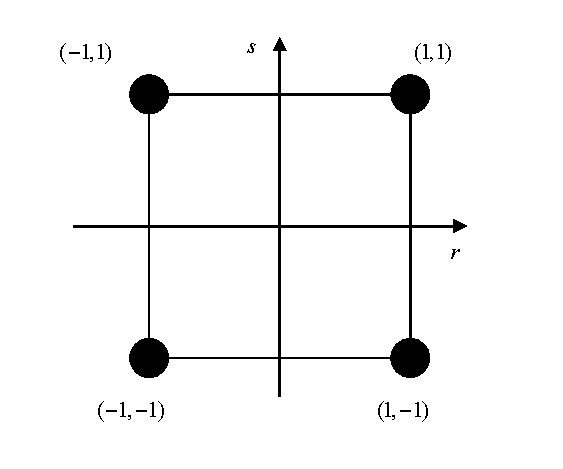
\includegraphics[width=6cm]{img/figure3.pdf}
\caption{Natural domain of integration}
\label{fig:Nat domain}
\end{figure}	 		
 

Once the interpolator $\hat{B}_{ij}^K(\vec{r})$ has been identified the elemental stiffness matrix is obtained via numerical integration (quadrature) as described in \eqref{eq:eleinetgration};

\begin{equation}
\int\limits_{r=-1}^{r=+1}\int\limits_{s=-1}^{s=+1} \hat{B}_{ij}^K(r,s) C_{ijkl} \hat{B}_{kl}^P(r,s)J(r,s) \mathrm{d}r\mathrm{d}s\approx \sum_{i,j=1}^\text{NGPTS} \alpha_i \alpha_j \hat{B}_{kl}^K(r_i,s_j)C_{ijkl} \hat{B}_{kl}^P(r_i,s_j) J(r_i,s_j)
\label{eq:eleintegration}
\end{equation}

	 											
and where NGPTS corresponds to the number of integration points, $\alpha_j$ is a weighting factor and $r_i,s_j$   are the coordinates of a typical point $\vec{r}$ in the natural space of \cref{fig:Nat domain}.

 
\begin{figure}[h]
\centering
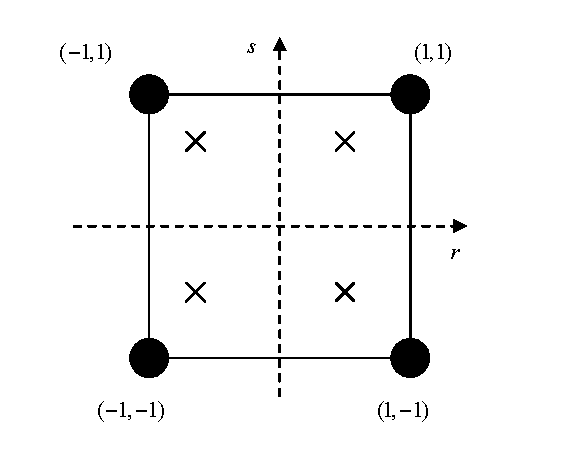
\includegraphics[width=6cm]{img/figure4.pdf}
\caption{Natural integration domain showing quadrature evaluation nodes}
\label{fig:integration domain}
\end{figure}	 


One important aspect of the numerical integration that has to be kept in mind is accuracy.  Depending on the particularly selected integration scheme, the number of introduced integration points fixes the maximum polynomial order of the considered functions that can be integrated accurately.  In the case of the integrand in \cref{eq:eleintegration}, it is clear that this order increases as the distortion of the physical element  with respect to the natural element increases.  One way of dealing with this dependency of accuracy with element distortion is to make use of adaptative integration techniques which are numerically expensive.  What is actually done in standard FEM analysis is to choose the number of quadrature points beforehand and introduce distortion related error criteria inside the code in such a way that some sort of validation is performed before the numerical integration process is started.

\section*{Strain displacement interpolator for the infinitesimal strain tensor}
The $Q$-th nodal contribution to the infinitesimal strain-displacement interpolator can be obtained in explicit form as follows. Let $L_x^Q$ and $L_y^Q$ be the spatial differential operators in $x$ and $y$ respectively. We have after expanding \cref{eq:fundamental interpolator}
%
\begin{align*}
L_x^Q & = J_{xP}^{-1}\frac{\partial N^Q}{\partial r_P} \equiv J_{xr}^{-1}\frac{\partial N^Q}{\partial r} + J_{xs}^{-1}\frac{\partial N^Q}{\partial s}\\
L_y^Q & = J_{yP}^{-1}\frac{\partial N^Q}{\partial r_P} \equiv J_{yr}^{-1}\frac{\partial N^Q}{\partial r} + J_{ys}^{-1}\frac{\partial N^Q}{\partial s}
\end{align*}
%
or in matrix form
%
\begin{equation}
\begin{Bmatrix}
L_x^Q\\
L_y^Q
\end{Bmatrix} = 
\begin{bmatrix}
J_{xP}^{-1} &J_{xs}^{- 1}\\
J_{yr}^{-1} &J_{ys}^{- 1}
\end{bmatrix}
\begin{Bmatrix}
\frac{\partial N^Q}{\partial r}\\
\frac{\partial N^Q}{\partial s}
\end{Bmatrix}
\end{equation}

The $Q$-th nodal contribution is then assembled as follows;


\begin{equation}
\begin{Bmatrix}
\frac{\partial u}{\partial x}\\
\frac{\partial v}{\partial y}\\
\frac{\partial u}{\partial y} + \frac{\partial v}{\partial x}
\end{Bmatrix} =
\begin{bmatrix}
 &L_x^Q &0 \\
\cdots &0 &L_y^Q &\cdots\\
 &L_y^Q &L_{xy}^Q
\end{bmatrix}
\begin{Bmatrix}
\vdots\\
u^Q\\
v^Q\\
\vdots
\end{Bmatrix}
\label{eq:strain inter}
\end{equation}

\begin{algorithm}[H]
\SetAlgoLined
\KwData{Nodal coordinates $x^Q$}
\KwResult{Strain-displacement interpolator $B_{ij}^Q$ }
Compute Jacobian ${J_{iJ}} = \frac{{\partial N_i^Q}}{{\partial {r_J}}}{{\hat x}^Q}$\\
Invert Jacobian  ${J_{iJ}} \to J_{iJ}^{ - 1}$\\
Compute fundamental interpolator $L_{ij}^Q = J_{jP}^{ - 1}\frac{{\partial N_i^Q}}{{\partial {r_P}}}$\\
Assemble $B_{ij}^Q = \frac{1}{2}\left( {L_{ij}^Q + L_{ji}^Q} \right)$ 
\caption{Strain-displacement interpolator}
\end{algorithm}


